\documentclass[10pt,pdf,hyperref={unicode}]{beamer}
\usepackage{amsmath, amsfonts}
\usepackage[utf8]{inputenc}
\usepackage[russian]{babel}
\usepackage{graphicx}
\usepackage{subcaption}
\usetheme{Warsaw}

\DeclareMathOperator{\svert}{\,\vert\,}
 
\setbeamertemplate{footline}[page number]{}
\setbeamertemplate{navigation symbols}{}

\usepackage[labelsep=period]{caption}
\addto\captionsrussian{\renewcommand{\figurename}{Рисунок}}

\hypersetup{pdfpagemode=FullScreen}
\author{Ефим Пышнограев}
\date{22 мая 2014}
\institute{Филиал МГУ в городе Севастополе}
\title{Извлечение описаний событий предопределённых типов из потока сообщений пользователей микроблогов}

\begin{document}

\begin{frame}
  \titlepage
\end{frame}

\begin{frame}
 \frametitle{Задача извлечения событий}
 Входные данные:
 \begin{itemize}
 \item набор коротких сообщений пользователей,
 \item каждое сообщение состоит из текста, автора и временной метки.
 \end{itemize}
 Найти:
 \begin{itemize}
 \item набор событий,
 \item событие --- ключевые слова и время возникновения.
 \end{itemize}
 Особенности сети Твиттер:
 \begin{itemize}
 \item небольшая длина сообщений,
 \item большое количество шума,
 \item высокая плотность сообщений,
 \item ``взрывной'' характер событий.
 \end{itemize}
\end{frame}

\begin{frame}
 \frametitle{Цели дипломной работы}
 Дипломная работа ставит перед собой следующие цели:
 \begin{itemize}
 \item исследовать существующие подходы к задаче извлечения событий,
 \item исследовать возможность применения тематических моделей для решения задачи выявления событий,
 \item разработать метод для извлечения событий из сообщений пользователей сети Твиттер на основе иерархического процесса Дирихле,
 \item оценить качество работы алгоритма.
 \end{itemize}	 
\end{frame}

\begin{frame}
  \frametitle{Схема алгоритма}
  Составные части:
  \begin{enumerate}  
  \item нахождение максимумов частотной функции, в которых будет производиться поиск событий,
  \item[] для каждого максимума:
   \item извлечение ключевых слов, характерных найденному максимуму,
   \item применение модели HDP с частичным обучением для того чтобы выделить все сообщения, которые соответствуют найденным ключевым словам,
   \item проверка, являются ли найденные ключевые слова и момент времени событием.
  \end{enumerate}
\end{frame}

\begin{frame}
  \frametitle{Используемые данные}
  Данные: 240 тысяч сообщений с 4 июня по 1 июля 2013 года, содержащие хэштег \#texas.
    \begin{figure}[H]
  \centering
  \begin{subfigure}[b]{0.45 \textwidth}
	  \centering
	  \includegraphics[width=5.0cm]{all-freq.eps}
%	  \caption*{а)}
  \end{subfigure}
  \begin{subfigure}[b]{0.45 \textwidth}
	  \centering
	  \includegraphics[width=5.0cm]{all-freq-scaled.eps}
%	  \caption*{б)}
  \end{subfigure}  
  \caption{Количество сообщений в час.}
	\end{figure}
\end{frame}

\begin{frame}
\frametitle{Работа алгоритма}
 Шаг 1: выделение экстремумов.
 \begin{figure}[H]
  \centering
  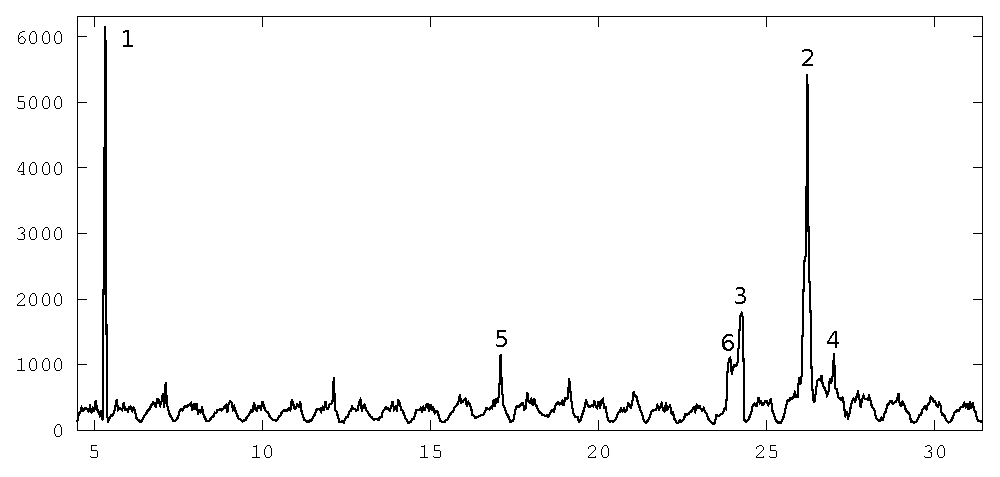
\includegraphics[width=10.0cm]{all-freq-labeled-1.eps}
  \label{fig:all-freq-labeled}
 \end{figure}
\end{frame}

\begin{frame}
\frametitle{Работа алгоритма}
Шаг 2: выделение ключевых слов.
\begin{table}
\begin{tabular}{r | l}
1 & year, read, prison, dragon, amazon, \\
2 & sb5, standwithwendi, talk, made, histori \\
3 & houston, california, england, artist, rt \\
4 & execut, 500th, mccarthi, kimberli, 1976 \\
5 & florida, z1, america, usa, bahrain \\
6 & houston, california, rt, watch, england \\
\end{tabular}
\end{table}	
\end{frame}

\begin{frame}
\frametitle{Работа алгоритма}
Шаг 3,\ 4: применение модели HDP, фильтрация:
\begin{itemize}
\item на основе частоты сообщений, принадлежащих событию:
\begin{figure}[H]
\centering
\begin{subfigure}[b]{0.45 \textwidth}
	  \centering
	  \includegraphics[width=5.0cm]{all-freq-27-0-1.eps}	
  	  \caption*{а) событие}
  \end{subfigure}
  \begin{subfigure}[b]{0.45 \textwidth}
	  \centering
	  \includegraphics[width=5.0cm]{all-freq-17-2-1.eps}	
  	  \caption*{б) не событие}
  \end{subfigure}
\end{figure}
\item на основе отношения количества уникальных авторов к числу сообщений.
\end{itemize}
\end{frame}

\begin{frame}
\frametitle{Работа алгоритма}
{\small
\begin{table}[H]
\centering		
\begin{tabular}{| l | l |}
	\hline
	 Ключевые слова & Событие \\ \hline
	 \begin{tabular}{l} year, read, prison, dragon, \\ amazon, written, bestseller \end{tabular} & \begin{tabular}{l} Написанная в техасской тюрьме книга \\ The Sword and the Dragon является \\ бестселлером на Amazon уже более трех \\ лет. \end{tabular} \\ \hline
	 \begin{tabular}{l} sb5, standwithwendi, abort, \\ senat \end{tabular} & \begin{tabular}{l} Обсуждение сенатом закона по запрету \\ абортов, который носит название Senate \\ Bill 5. Wendi Davis ---  политик, которая \\ боролась с принятием этого закона.  \end{tabular} \\ \hline
	 \begin{tabular}{l} execut, 500th, mccarthi, \\ kimberli, 1976\end{tabular} & \begin{tabular}{l} В штате Техас приведен в исполнение \\ 500-й по счету смертный приговор. \\ Смертная казнь имеет место с 1976 года.\end{tabular} \\ \hline
	\end{tabular}
\end{table}
}
\end{frame}

\begin{frame}
  \frametitle{Оценка качества}
  Для оценки качества было сделано предположение:
  \begin{itemize}
  \item если данные содержат событие, оно находится в максимуме функции частоты.
  \end{itemize}
  
  Сравнение с базовым алгоритмом New event detection:
  	\begin{table}[h]
	\centering
	\begin{tabular}{ l l l l}
	Алгоритм & Точность & Полнота & F-мера \\ \hline
	предложенный алгоритм  & 0.8 & 1.0 & 0.89 \\ 
	New event detection & 0.01 & 0.8 & 0.02 \\ 
	\end{tabular}
		\caption{Оценка качества исходя из предположения}
	\end{table}
	
	Почему у NED такая низкая точность на данных Твиттера:
	\begin{itemize}
	\item большая плотность новых слов из-за шума в данных,
	\item предположение, сделанное для оценки качества.
	\end{itemize}
	
\end{frame}

\begin{frame}
  \frametitle{Детали оценки качества}
  Пусть:
  \begin{itemize}
  \item $n$ событий было выдано алгоритмом,
  \item $m$ событий находится во входных данных,
  \item $k$ событий были верно найдены алгоритмом.
  \end{itemize}
  
  Критерии качества:
  \begin{itemize}
  \item точность $p = k/n$,
  \item полнота $r = k/m$,
  \item F-мера $F = 2pr/(p+r)$.
  \end{itemize}
  
  Способ оценки:
  \begin{itemize}
  \item точность: просмотреть $n$ сообщений и выделить верные события,
  \item полнота: 
  \begin{itemize}
  \item с предположением об экстремумах: просмотреть небольшое количество максимумов функции частоты,
  \item без предположения: просмотреть все сообщения для выделения событий.
  \end{itemize}
  \end{itemize}
  
\end{frame}

\begin{frame}
  \frametitle{Заключение}
  В ходе выполения дипломной работы было достигнуто:
	\begin{itemize}
	 \item исследованы существующие подходы к задаче извлечения событий,
	 \item исследованно и продемонстрировано применение тематических моделей для решения задачи,
	 \item разработан метод для извлечения событий из сообщений пользователей сети Твиттер на основе иерархического процесса Дирихле,
	 \item изучено качество работы предложенного алгоритма на имеющихся данных.
	\end{itemize}
\end{frame}

\end{document}
